% As técnicas existentes implementadas serão executadas usando os {\it benchmarks} usuais como o SPEC, e serão escolhidos {\it benchmarks} que simulam o ambiente real de utilização de máquinas virtuais. Serão feitas modificações nas técnicas para melhorar o desempenho nas máquinas virtuais principalmente utilizando os {\it benchmarks} escolhidos. Se preciso, também serão propostas e implementadas novas técnicas de formação de regiões, onde o resultado esperado é que estas também tenham um melhor desempenho principalmente nos {\it benchmarks} que simulam o ambiente real.

  
  For fault injection and performance evaluation, we will use Gaisler's debugging interface GRMON which is a general debug monitor for the LEON processor, and for SOC designs based on the GRLIB IP
library. GRMON includes the following functions:
\begin{itemize}

 \item Read/write access to all system registers and memory
 \item Built-in dis-assembler and trace buffer management
 \item Downloading and execution of LEON applications
 \item Breakpoint and watchpoint management
 \item Remote connection to GNU debugger (GDB)
 \item Support for USB, JTAG, RS232, PCI, Ethernet and SpaceWire debug links

\end{itemize}
 
\subsection{ GRMON Debug Monitor}

The GRMON debug monitor is intended to debug system-on-chip (SOC) designs based on the LEON processor. 
The monitor connects to a dedicated debug interface on the target hardware, through which it can perform
read and write cycles on the on-chip bus (AHB). The debug interface can be of various types: the LEON2 processor
supports debugging over a serial UART and 32-bit PCI, while LEON3 also supports JTAG, ethernet and
spacewire debug interfaces. On the target system, all debug
interfaces are realized as AHB masters with the debug protocol implemented in hardware. There is thus no
software support necessary to debug a LEON system, and a target system does in fact not even need to have a
processor present.

 \begin{figure}[ht]
    \centering
    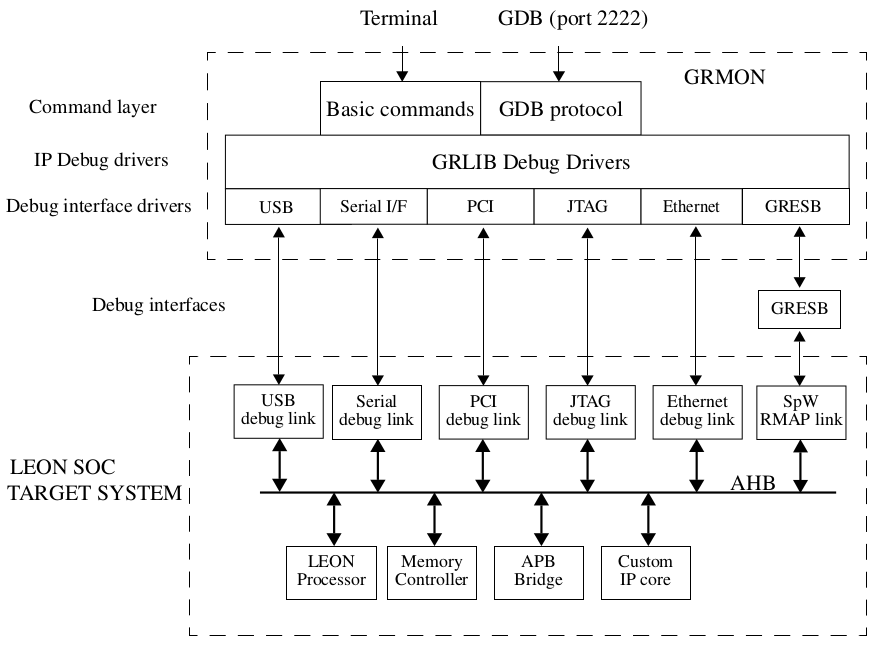
\includegraphics[width=0.75\textwidth]{figures/grmon_ex.png}
    \caption{GRMON  Interface }
    \label{fig:grmon_int}
\end{figure}
GRMON can operate in two modes: command-line mode and GDB mode. In command-line mode, GRMON
commands are entered manually through a terminal window. In GDB mode, GRMON acts as a GDB gateway
and translates the GDB extended-remote protocol to debug commands on the target system.
GRMON is implemented using three functional layers: command layer, debug driver layer, and debug interface
layer. The command layer consist of a general command parser which implements commands that are independent
of the used debug interface or target system. These commands include program downloading and flash
programming.
The debug driver layer implements custom commands which are related to the configuration of the target system. 
GRMON scans the target system at start up, and detects which IP cores are present and how they are con-
figured. For each supported IP core, a debug driver is enabled which implements additional debug commands
for the specific core. Such commands can consist of memory detection routines for memory controllers, or program
debug commands for the LEON processors.
The debug interface layer implements the debug link protocol for each supported debug interface. The protocol
depends on which interface is used, but provides a uniform read/write interface to the upper layers. Which
interface to use for a debug session is specified through command-line options during the start of GRMON.

  \subsection{ Performance Analysis}
  \label{subsec:performance}

%    \begin{figure*}[!t]
% 	  \centering
% 	  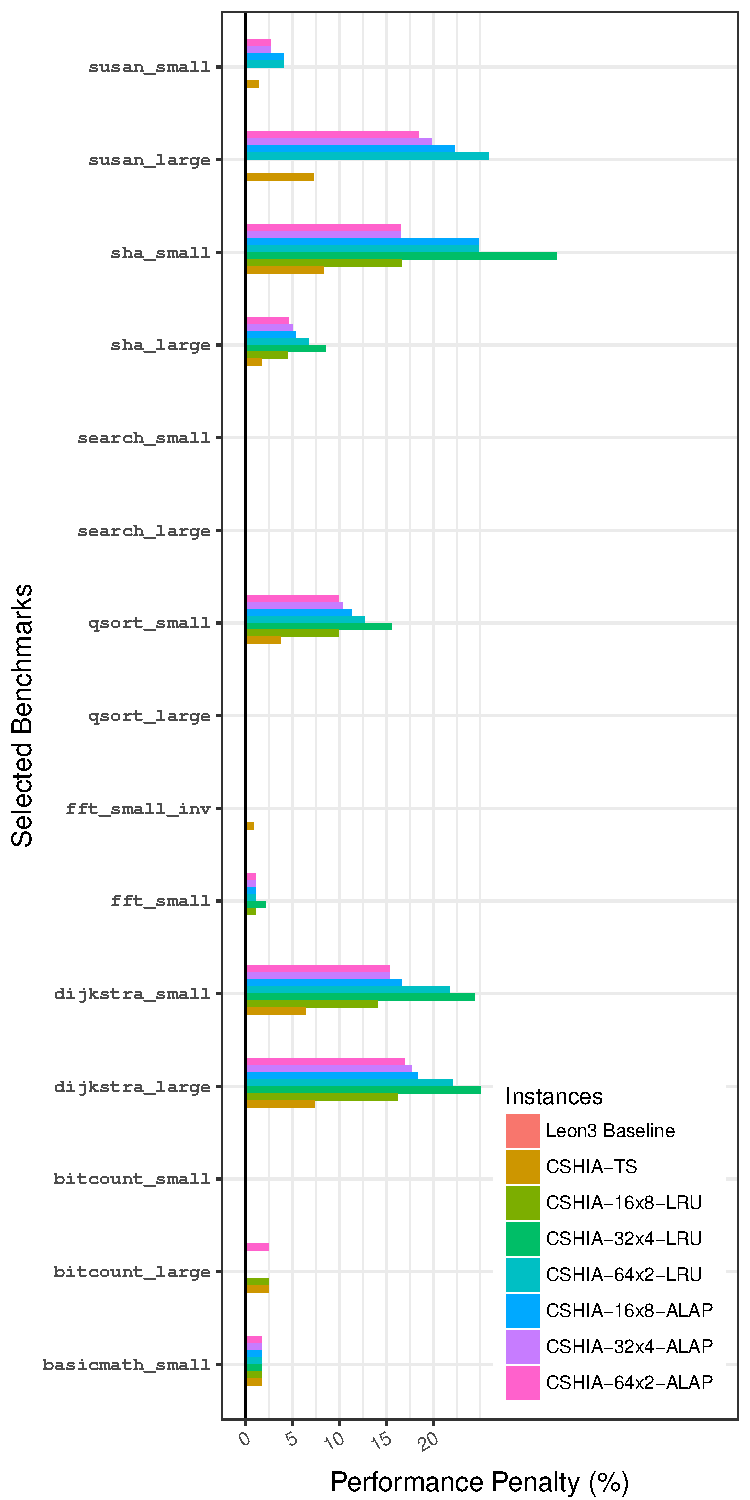
\includegraphics[scale=0.6]{benchmarks.pdf}
% 	  \caption{Execution time for benchmarks. For each benchmark, the running time was normalized by Leon's running time.}
%   %	\vspace*{-9pt} 
% 	  \label{fig:benchmarks}
%   \end{figure*}
  
  For correctness, the  \cshia~prototype will be  evaluated using 8 benchmarks from the MiBench suite: \texttt{basicmath}; \texttt{bitcount}; \texttt{crc32}; \texttt{dijkstra}; \texttt{fft}; \texttt{qsort}; \texttt{sha}; \texttt{stringsearch}. Benchmark outputs will be compared to the outputs of reference execution of MiBench and also to those produced by the Leon baseline implementation. In addition, program performance will be compared among three architectures: (1) Unmodified Leon 3 (baseline); (2) \cshia~(unsecured), whose authentication and integrity verification will be disabled by making the bus traffic bypass the \seccache; and (3) \cshia~(secure), the architecture proposed herein. All architectures will use a 50-MHz clock, 16-KB L1 data and instruction caches with 256-bit cache lines.

  As Leon 3 (baseline), and consequently both \cshia~(unsecured) and \cshia~(secure), do not support system calls, benchmarks that read files will be modified to obtain their data from hard-coded integer or string vectors. Large MiBench inputs will be used for all benchmarks.
  %, except by \texttt{basicmath} and \texttt{fft}.   The \ptag~Memory was set to 4096 64-bit \ptags, which covers 128 KB of main memory, from the beginning of the text memory segment (\texttt{0x40000000}) until after the data memory segment (\texttt{0x4001FFFF}) of the programs. This coverage was enough for almost all benchmarks but \texttt{crc32}, \texttt{qsort}, and \texttt{sha}. These were only partially covered because hard-coding their inputs oversized their binary code, demanding a bigger \ptag~Memory, which could not fit into our current \fpga~design. For the same reason, both stack and heap memory segments of the programs were also not covered.

%   Figure \ref{fig:benchmarks} shows an overal performance degradation of \cshia~(secure) below 10\% in 5 benchmarks. The \texttt{crc32}, \texttt{dijkstra}, and \texttt{sha} benchmarks had penalties of 13\%, 17\%, and 39\%, respectively. Comparing \texttt{crc} and \texttt{sha} performances on \cshia~(unsecured) and \cshia~(secure), one can see that the degradation is not related to integrity verification but to \fpga~synthesis issues instead. Since \cshia~(unsecured) does not verify \ptags~or buffer memory blocks, performance should have been similar to the Leon (baseline). Even though we have not performed a detailed analysis, a non-optimal synthesized design may have played a major factor on the performance degradation. If it were possible to mitigate the performance gap between Leon 3 (baseline) and \cshia~(unsecured), \cshia~(secure) would present a very small overhead performance since the biggest difference between \cshia~(unsecured) and \cshia~(secure) happened in the \texttt{dijkstra} benchmark which has only a 9\% penalty. Identifying the issue involved in the \cshia~(unsecure) bypass hardware is in progress.
%   
%   Achieving an optimal design involves many variables that play positively or negatively in the prototype's performance. Full main memory coverage may impose performance penalties, but then again, a proper size of the \seccache can compensate for that. Overall, \cshia~seems to represent an interesting secure architecture, providing code and data authenticity and integrity with an average 13\% of performance overhead for the executed benchmarks.

  \subsection{Fault Injection Attack}
  \label{subsec:attack}
  
  
  Many attack scenarios proposed in~\cite{Hoffman2015}  can be used to evaluate the \cshia prototype, in most of them the attack is performed by inserting a modified memory block into the bus or main memory. Thus, verifying how those insertions can happen and how they will affect the behavior of \cshia~is crucial. This section presents an execution of a fault injection attack planned to be executed in the real prototype. 


\begin{figure}[!hbt]
	\centering
  \begin{minipage}[c]{0.6\linewidth}
	\lstinputlisting[language=c, tabsize=1, numbers=right, numbersep=-5pt, firstline=126, lastline=135, basicstyle=\footnotesize]{figures/sha.c}
	\caption{C code for the \texttt{sha} initialization function.}
%	\vspace*{-9pt} 
	\label{fig:c-code}
\end{minipage}
\end{figure}

% 	\vspace*{1cm} 

\begin{figure}[!thb]
	\centering
  \begin{minipage}[c]{0.6\linewidth}	\lstinputlisting[language={[x86masm]Assembler}, tabsize=1, numbers=right, numbersep=-5pt, firstline=2055, lastline=2056, basicstyle=\footnotesize]{figures/sha.objdump}
	\caption{SPARC assembly code where the constant \texttt{0x67452301} is assigned to a global register.}
%	\vspace*{-9pt} 
	\label{fig:assembly}
	\end{minipage}

\end{figure}




  The attack scenario is the following. An attacker wants to tamper with the message integrity scheme of a node from a sensor network. The Secure Hash Algorithm (SHA) is used in this network to create a \textit{Message Authentication Code} (MAC) for incoming and outgoing messages. The goal of the attacker is to make a particular node reject all incoming messages with valid MACs and generate invalid MACs for outgoing messages that all other nodes will reject. This attack may be hard to detect since all nodes will be active and promptly responding, but the network is malfunctioning. 
% 
%   This attack has been applied to program \texttt{sha} in all tree evaluated architectures. Given the limited coverage of the \cshia~prototype, we selected a critical part of the algorithm to attack in the memory range of \texttt{0x40000000} to \texttt{0x4001FFFF}. 
For fault injection, we will use Gaisler's debugging interface, GRMON, to directly insert memory words into the AMBA bus. Faults will be inserted as bus memory write operations that can be executed during the runtime of a program, after a breakpoint. An attacker could easily achieve that by connecting a physical adapter to the external pins of the processor.
% 
   As implementations of SHA are open, we assume the attacker knows all the source code and decides to tamper with the initialization process, in which constant values are assigned, as shown in Figure \ref{fig:c-code}. The attacker then learns that line 3 from Figure \ref{fig:c-code} is compiled to the two instructions in Figure \ref{fig:assembly}. Given that, \attacker~replaces the memory word \texttt{05 19 d1 48}, a \texttt{sethi} instruction, by \texttt{05 11 11 11}, which represents the substitution of constant \texttt{0x67452301} by \texttt{0x44444701}. After applying the attack, all digest values will differ from those generated by an authentic implementation of SHA. This initial scenario will be used to evaluate the \cshia prototype.
% 
%   After applying the above mentioned attack to the insecure architectures Leon 3 (Baseline) and \cshia~(unsecured), the attacker succeeds and the attack goes undetected: \texttt{sha} takes MiBench's large reference input and produces an output different from the correct reference output. On the other hand, \cshia~(secure) stops the execution at address \texttt{0x40001f84}, which is the location of the tampered instruction, and no further instructions are executed. By stopping the execution in a NMI state, \cshia~(secure) enables a fast detection of the security violation in the sensor network. Therefore, tamper-evidence and tamper-resistance were provided by \cshia. 

